%06chapterVergleich.tex

\chapter{Vorgehen}
\label{sec:Vorgehen}

Als Pascal die ganze Koordination übernahm, erstellte er anfangs ein Grobablauf \ref{fig:grobablauf}, der uns als Grundlage und gute Übersicht dienen sollte.

\begin{figure}[ht]
	\centering
	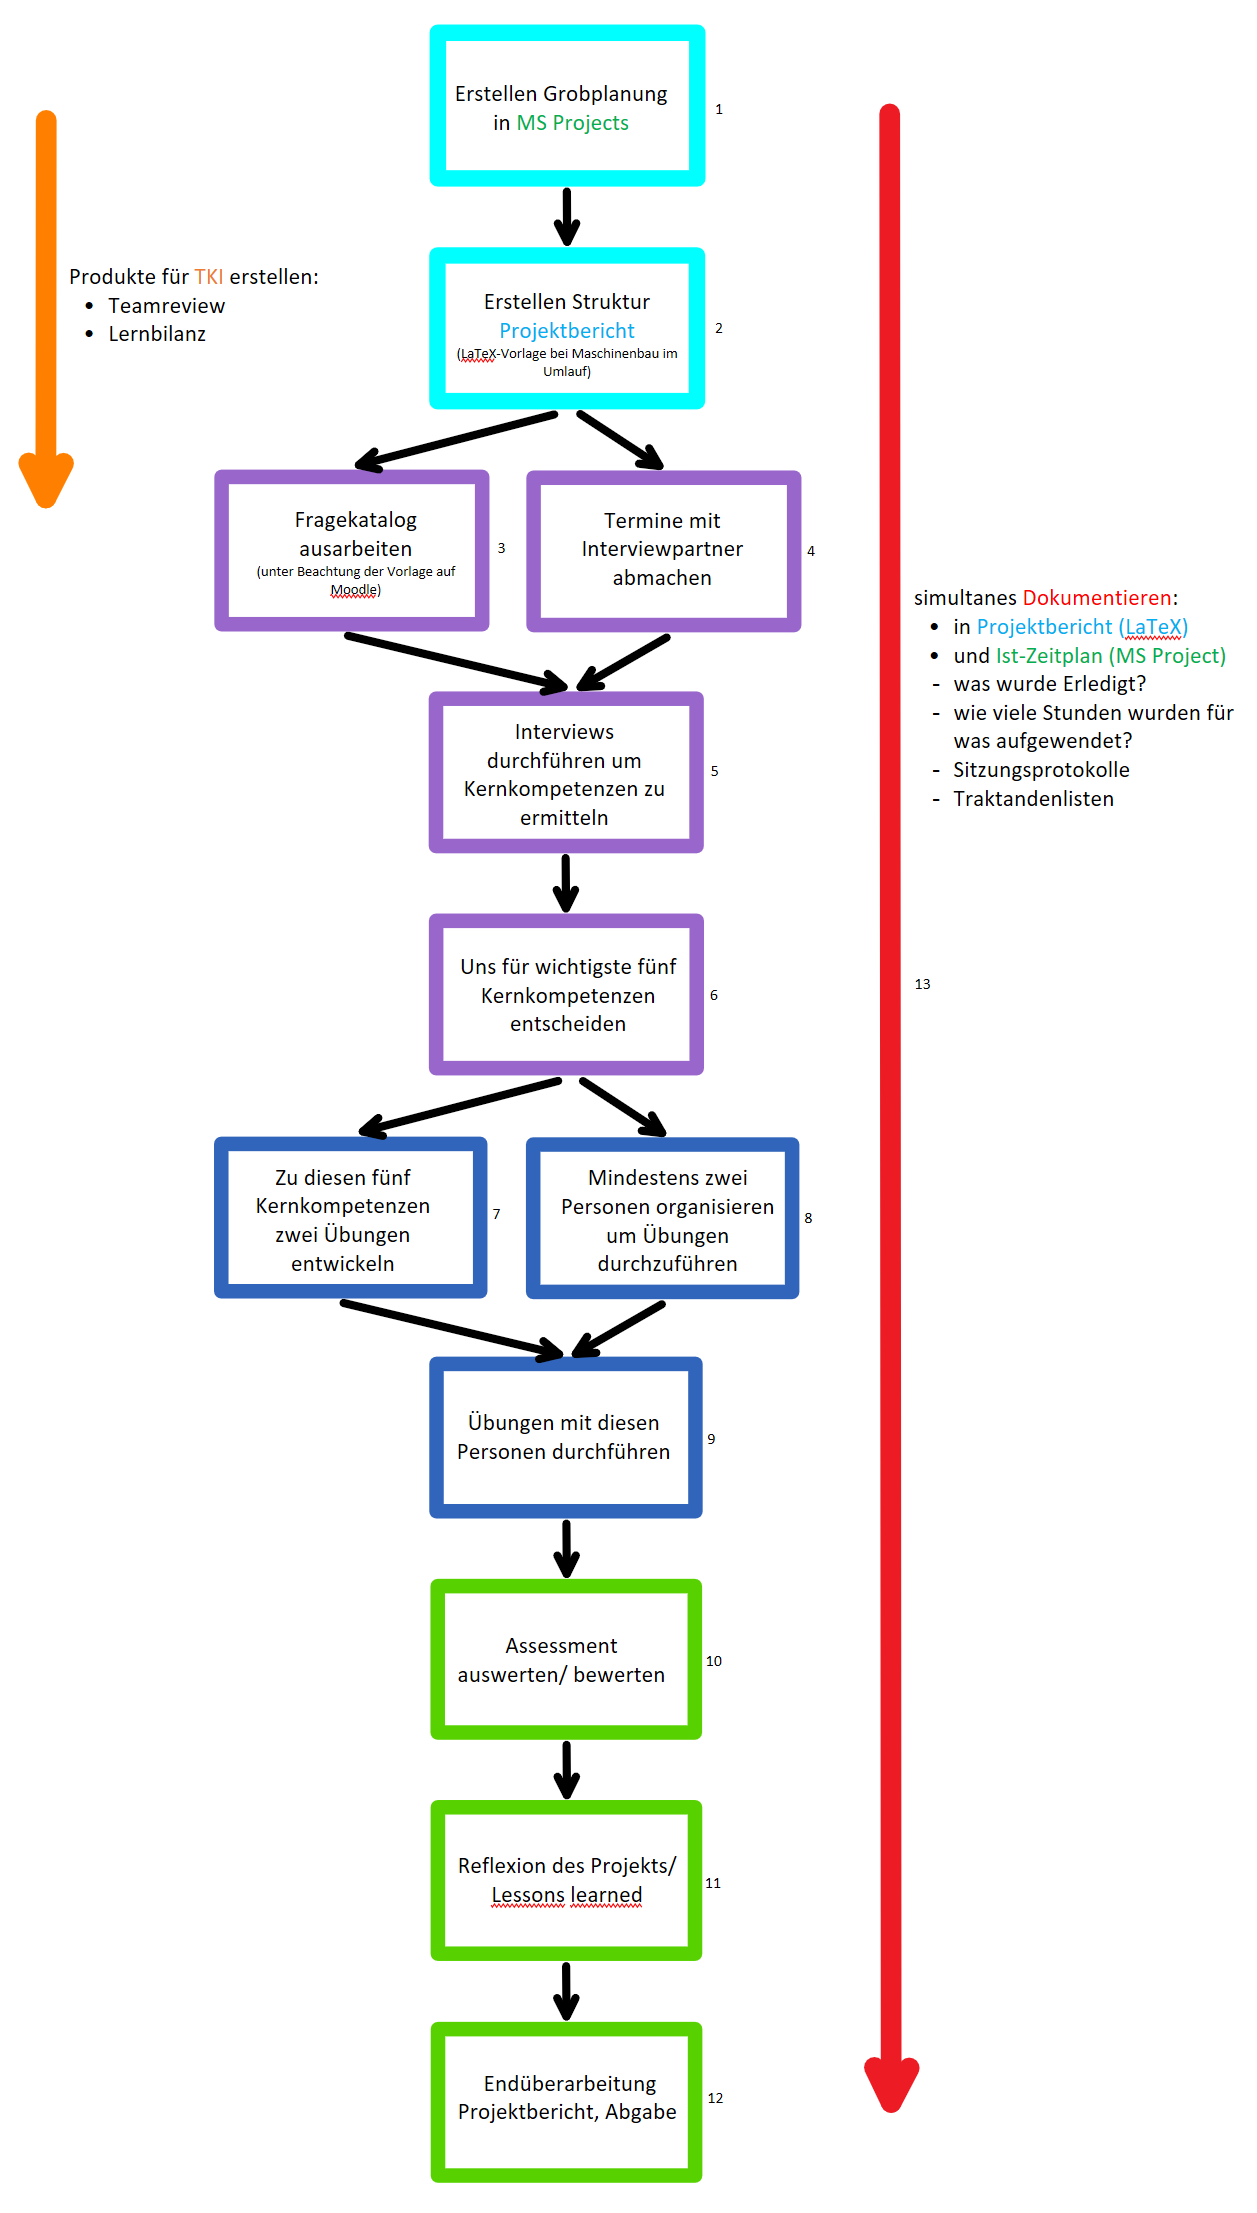
\includegraphics[width=0.9\textwidth]{images/Grobablauf.png}
	\caption{Grobablauf}
	\label{fig:grobablauf}
\end{figure}

Anschiessend hat er mittels MS Project eine Detailplanung \ref{fig:msproject} erstellt. Diese enthält alle Arbeiten inkl. Zeitvorgaben.

\begin{figure}[ht]
	\centering
	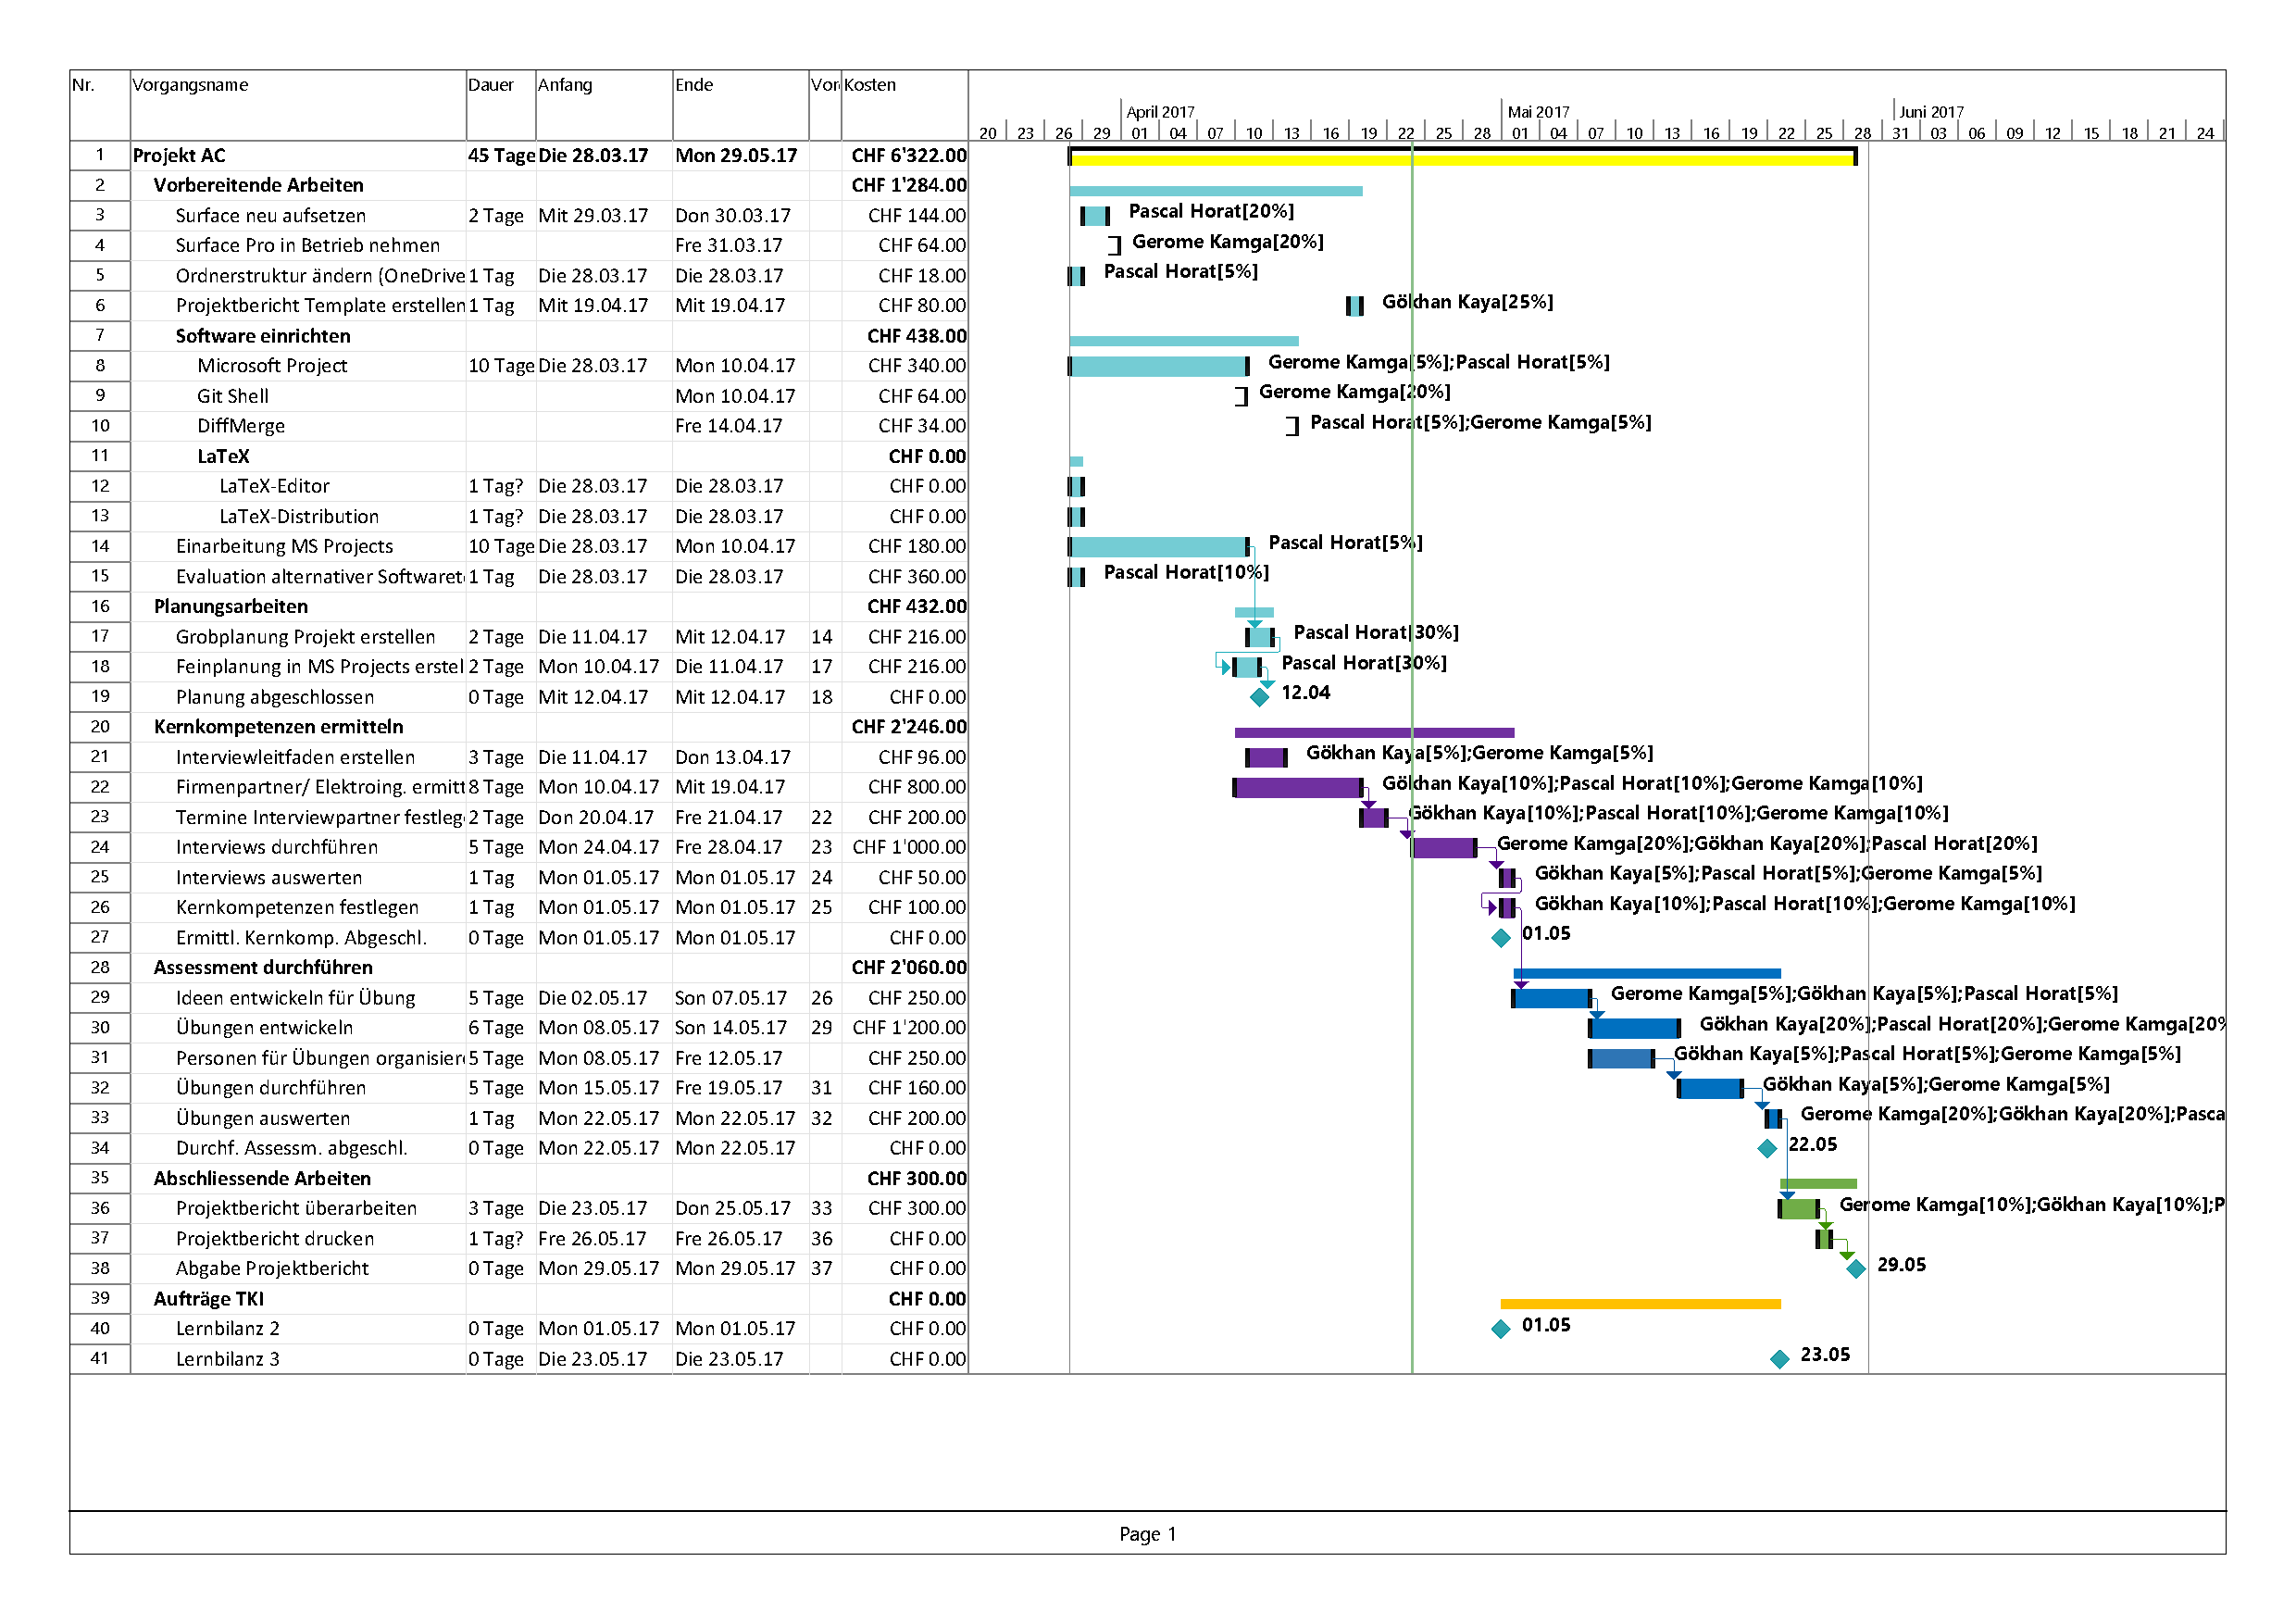
\includegraphics[width=1.6\textwidth, angle =270]{images/BaselineAC2.pdf}
	\caption{Baseline in MS Project}
	\label{fig:msproject}
\end{figure}

Um die Aufträge koordinieren zu können, hat Pascal schliesslich ein Excel-File erstellt und diese auf One-Drive geladen. Dieses File liess sich von allen (jedoch nicht Gleichzeitig) online bearbeiten und abspeichern. Pascal konnte nach den Fristen seine Kommentare dazu abgeben oder falls nötig dazu auffordern einige Korrekturen vorzunehmen. Je nach Stand der Arbeit wurden die Aufträge gemäss Bild \ref{fig:auftrage} farblich markiert. Gökhan und Gerome konnten jeweils eintragen, wie viel der Aufträge (in Prozente) bereits erledigt und wieviel Zeit dafür aufgewendet wurde. 

\begin{figure}[ht]
	\centering
	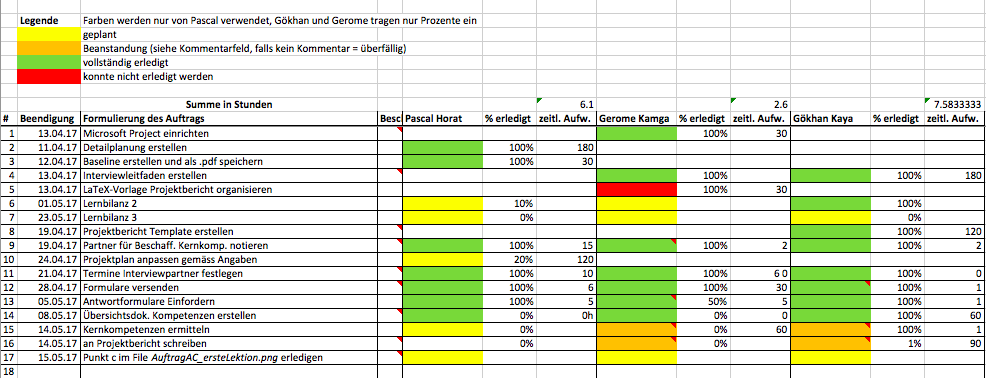
\includegraphics[width=1.1\textwidth]{images/Auftrage}
	\caption{Ausschnitt Auftragsaufteilung}
	\label{fig:auftrage}
\end{figure}

Da viele Arbeiten mittels dem Versionsverwaltungstool Git erledigt wurden, kann an dieser Stelle ebenfalls eine gute Übersicht über die tatsächlich erledigten Arbeiten gezeigt werden. Aufgrund der Grösse dieser Commit History ist sie im Anhang unter REFERENZ aufgeführt DIESER SATZ AUCH IN ANHANG --> Unten ist die Liste mit unseren tatsächlich hochgeladenen Änderungen inkl. unseren Kommentaren zu sehen.

